\documentclass[tikz]{standalone}
\usepgflibrary{arrows.meta}
\usepackage{xcolor}
\begin{document}
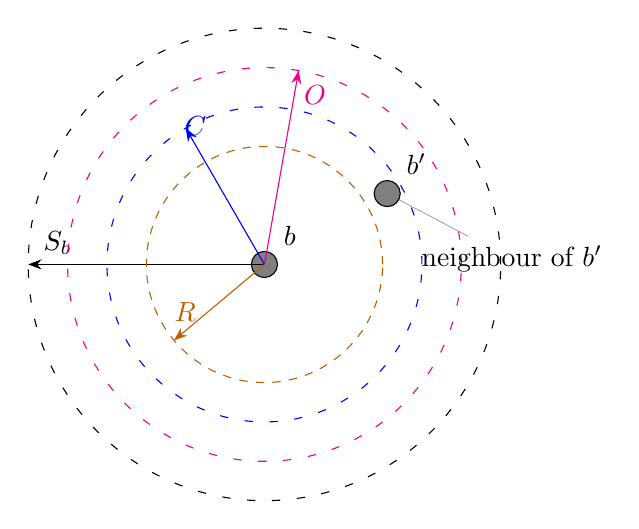
\begin{tikzpicture}[>=Stealth]
\node[circle,fill=black!50,draw,label=above right:$b$]{};

  \draw[loosely dashed,radius=3cm,draw] (0,0) circle;
  \draw[->] (0,0)-- node[very near end,above]{$S_b$} (180:3cm);

  \draw[loosely dashed,radius=2.5cm,draw=magenta] (0,0) circle;
  \draw[->,magenta] (0,0)-- node[very near end,right]{$O$} (80:2.5cm);
  
  \draw[loosely dashed,radius=2cm,draw=blue] (0,0) circle;
  \draw[->,blue] (0,0)-- node[very near end,above]{$C$} (120:2cm);
  
  \draw[dashed,radius=1.5cm,draw=orange!75!black] (0,0) circle;
  \draw[->,orange!75!black] (0,0)-- node[very near end,above]{$R$} (220:1.5cm);

  \node at (30:1.8cm) [circle,fill=black!50,draw,label=above right:$b^\prime$,
  	pin distance=2cm,pin=300:{neighbour of $b'$}]{};
\end{tikzpicture}
\end{document}

